\section{Vektor dalam $\mathbb{R}^n$}

\begin{outcome}

\begin{enumerate}
\item[A.] Menentukan vektor posisi suatu titik dalam $\mathbb{R}^n$.
\end{enumerate}
\end{outcome}

Notasi $\mathbb{R}^{n}$ mengacu pada kumpulan daftar terurut yang terdiri atas
$n$ bilangan real, yaitu
\[
\mathbb{R}^{n} = \left\{ \left( x_{1}\cdots x_{n}\right)
:x_{j}\in \mathbb{R}\text{ untuk }j=1,\cdots ,n\right\}
\]
Dalam bab ini, kita akan menelaah vektor dalam $\mathbb{R}^n$ secara lebih mendalam. Pertama-tama, kita akan meninjau dengan lebih terperinci seperti apa
$\mathbb{R}^n$ itu. Ingat bahwa titik yang diberikan oleh $0=\left( 0, \cdots, 0 \right)$ disebut \textbf{titik asal}.

Sekarang, perhatikan kasus $\mathbb{R}^n$ untuk $n=1.$ Dari definisi tersebut, kita dapat mengidentifikasi
$\mathbb{R}$ dengan titik-titik dalam $\mathbb{R}^{1}$ sebagai berikut:
\begin{equation*}
\mathbb{R} = \mathbb{R}^{1}=
 \left\{ \left( x_{1}\right) :x_{1}\in \mathbb{R} \right\}
\end{equation*}
Jadi, $\mathbb{R}$ didefinisikan sebagai himpunan semua bilangan real dan, secara geometris,
kita dapat menggambarkannya sebagai semua titik pada sebuah garis.

Sekarang misalkan $n=2$. Maka, dari definisi,
\begin{equation*}
\mathbb{R}^{2}=
\left\{ \left(x_{1}, x_{2}\right)
:x_{j}\in \mathbb{R}\text{ untuk }j=1,2 \right\}
\end{equation*}
Perhatikan bidang koordinat yang sudah dikenal, dengan sumbu $x$ dan sumbu $y$. Setiap titik
di dalam bidang koordinat ini diidentifikasi berdasarkan letaknya
di sepanjang sumbu $x$, dan juga berdasarkan letaknya di sepanjang sumbu $y$.
Sebagai contoh, perhatikan diagram berikut.

\begin{center}
\begin{tikzpicture}
\draw[<->](-4,0)--(4,0);
\draw[<->](0,-1)--(0,5);
\draw(2,0.2)--(2,-0.2);
\draw(-3,0.2)--(-3,-0.2);
\draw(-0.2,1)--(0.2,1);
\draw(-0.2,4)--(0.2,4);
\draw[help lines] (-3,0)--(-3,4)--(0,4);
\draw[help lines](0,1)--(2,1)--(2,0);
\draw[fill=red](-3,4) circle [radius=3pt];
\draw[fill=red](2,1) circle [radius=3pt];
\node[below right] at (4,0){$x$};
\node[left] at(0,5){$y$};
\node[below] at (-3,-0.5){$-3$};
\node[below] at (2,-0.5){$2$};
\node[left] at (-0.5, 1){$1$};
\node[left] at (-0.5, 4){$4$};
\node[above] at (-3,4){$Q = (-3,4)$};
\node[above] at (2,1){$P = (2,1)$};
\end{tikzpicture}\par\captionof{figure}{Plot dua dimensi bidang xy yang menunjukkan dua titik P = (2,1) dan Q = (-3,4) yang ditandai dengan warna merah...}\label{fig:RnVectorsRn-tikz01}% fig-num-auto

\end{center}

Dengan demikian, setiap elemen dalam $\mathbb{R}^2$ diidentifikasi oleh dua
komponen, $x$ dan $y$, dengan cara yang biasa. Koordinat $x, y$ (atau $x_1$,$x_2$) secara unik menentukan suatu titik pada bidang. Perhatikan bahwa walaupun definisi menggunakan $x_1$ dan $x_2$ untuk menamai koordinat dan Anda mungkin terbiasa dengan $x$ dan $y$, notasi-notasi ini setara.

Sekarang misalkan $n=3$. Anda mungkin sebelumnya pernah menjumpai sistem koordinat
$3$ dimensi, yang diberikan oleh
\begin{equation*}
\mathbb{R}^{3}=
\left\{ \left( x_{1}, x_{2}, x_{3}\right)
:x_{j}\in \mathbb{R}\text{ untuk }j=1,2,3 \right\}
\end{equation*}

Titik-titik dalam $\mathbb{R}^3$ ditentukan oleh tiga
koordinat, yang sering ditulis $\left(x,y,z\right)$ dan bersesuaian dengan sumbu $x$, $y$,
dan $z$. Seperti di atas, kita dapat menganggap bahwa dua koordinat pertama
menentukan sebuah titik pada bidang. Komponen ketiga menentukan
ketinggian di atas atau di bawah bidang, bergantung pada apakah bilangan ini
positif atau negatif, dan secara keseluruhan semuanya menentukan sebuah titik dalam
ruang. Anda dapat melihat bahwa tripel terurut bersesuaian dengan titik-titik dalam ruang, sebagaimana
pasangan terurut bersesuaian dengan titik-titik pada bidang dan bilangan real tunggal
bersesuaian dengan titik-titik pada garis.

Gagasan di balik $\mathbb{R}^n$ yang lebih umum adalah bahwa kita dapat memperluas
gagasan-gagasan ini melampaui $n = 3.$ Pembahasan mengenai titik-titik dalam $\mathbb{R}^n$ ini mengantar kita pada kajian vektor dalam $\mathbb{R}^n$. Walaupun kita membahas $\mathbb{R}^n$ untuk semua $n$,
pada bagian ini kita terutama akan berfokus pada $n=2,3$.

Perhatikan definisi berikut.

\begin{definition}{Vektor Posisi}\label{def:positionvector}
Misalkan $P=\left( p_{1},\cdots ,p_{n}\right) $ merupakan koordinat suatu
titik dalam $\mathbb{R}^{n}.$ Maka vektor $\longvect{0P}$ dengan pangkalnya di
$0=\left( 0,\cdots ,0\right) $ dan ujungnya di
$P$ disebut \textbf{vektor posisi} dari
\index{vektor posisi} \index{vektor!titik dan vektor} titik $P$.
Kita menulis
\begin{equation*}
\longvect{0P} = \leftB
\begin{array}{c}
p_{1} \\
\vdots \\
p_{n}
\end{array} \rightB
\end{equation*}
\end{definition}

Karena alasan ini, kita dapat menulis baik $P=\left( p_{1},\cdots ,p_{n}\right)  \in \mathbb{R}^{n}$
maupun $\longvect{0P} = \leftB p_{1} \cdots p_{n} \rightB^T \in \mathbb{R}^{n}$.

Definisi ini diilustrasikan pada gambar berikut untuk
kasus khusus $\mathbb{R}^{3}$.

\begin{center}
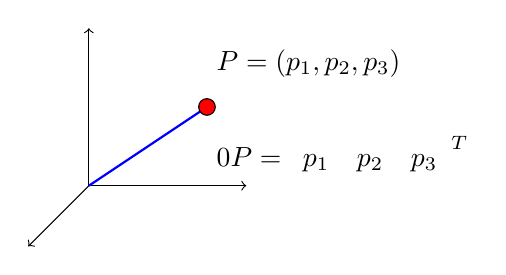
\begin{tikzpicture}
\draw[<->](2,0,0)--(0,0,0)--(0,2,0);
\draw[->](0,0,0)--(0,0,2);
\draw[thick, blue](0,0,0)--(1.5,1,0);
\draw[fill=red] (1.5, 1,0) circle [radius=3pt];
\node[above right] at (1.5, 1.25, 0){$P=(p_1, p_2, p_3)$};
\node[below right] at (1.5, 0.75, 0){$\longvect{0P}= \leftB \begin{array}{ccc}
p_1 & p_2 & p_3
\end{array}\rightB^T$};
\end{tikzpicture}\par\captionof{figure}{Diagram tiga dimensi vektor posisi 0P: sebuah panah biru tebal dari titik asal sepanjang...}\label{fig:RnVectorsRn-tikz02}% fig-num-auto

\end{center}

Jadi, setiap titik $P$ dalam $\mathbb{R}^{n}$ menentukan vektor posisinya
$\longvect{0P}$. Sebaliknya, setiap vektor posisi $\longvect{0P}$ semacam itu
yang berpangkal di $0$ dan berujung di $P$ menentukan titik $P$ dalam
$\mathbb{R}^{n}$.

Sekarang misalkan diberikan dua titik, $P,Q$, yang koordinatnya masing-masing adalah
$\left( p_{1},\cdots ,p_{n}\right) $ dan $\left(
q_{1},\cdots ,q_{n}\right) $. Kita juga dapat menentukan
\textbf{vektor posisi dari $P$ ke $Q$} (juga disebut \textbf{vektor dari $P$ ke $Q$}), yang didefinisikan sebagai berikut.
\begin{equation*}
\longvect{PQ} = \leftB \begin{array}{c}
q_{1}-p_{1}\\
 \vdots \\
q_{n}-p_{n}
\end{array}
\rightB = \longvect{0Q} - \longvect{0P}
\end{equation*}

Sekarang, bayangkan mengambil suatu vektor dalam $\mathbb{R}^n$ dan memindahkannya, dengan selalu
mempertahankan arah hadapnya seperti ditunjukkan dalam gambar berikut.

\begin{center}
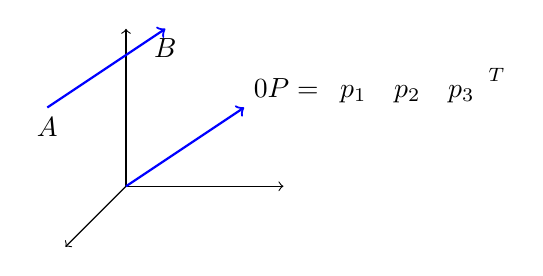
\begin{tikzpicture}
\draw[<->](2,0,0)--(0,0,0)--(0,2,0);
\draw[->](0,0,0)--(0,0,2);
\draw[->, thick, blue](0,0,0)--(1.5,1,0);
\draw[->, thick, blue](-1,1,0)--(0.5,2,0);
\node[right] at (1.5, 1.25, 0){$\longvect{0P}= \leftB \begin{array}{ccc}
p_1 & p_2 & p_3 \end{array}\rightB ^T$};
\node[below] at (-1,1,0){$A$};
\node[below] at (0.5,2,0){$B$};
\end{tikzpicture}\par\captionof{figure}{Diagram tiga dimensi dengan dua panah biru sejajar yang sama panjang dan searah: vektor posisi...}\label{fig:RnVectorsRn-tikz03}% fig-num-auto

\end{center}

Setelah dipindahkan, vektor itu tetap dianggap sebagai vektor yang sama. Setiap vektor, $\longvect{0P}$ dan $\longvect{AB}$, memiliki panjang (atau magnitudo) dan arah yang sama. Oleh karena itu, keduanya sama.

Sekarang perhatikan definisi umum untuk suatu vektor dalam $\mathbb{R}^n$.

\begin{definition}{Vektor dalam $\mathbb{R}^n$}\label{def:vectorsRn}
Misalkan $\mathbb{R}^{n} = \left\{ \left( x_{1}, \cdots, x_{n}\right)
:x_{j}\in \mathbb{R}\text{ untuk }j=1,\cdots ,n\right\} .$ Maka,
\begin{equation*}
\vect{x}
=
\leftB \begin{array}{c}
x_{1} \\
\vdots \\
x_{n}
\end{array}
\rightB
\end{equation*}
disebut sebuah \textbf{vektor}. Vektor memiliki besar (magnitudo) sekaligus arah.
Bilangan-bilangan $x_{j}$ disebut \textbf{komponen} dari $\vect{x}$.
\index{vektor!komponen}
\index{vektor}
\end{definition}

Dengan menggunakan notasi ini, kita dapat memakai $\vect{p}$ untuk menyatakan vektor posisi titik $P$. Perhatikan bahwa dalam konteks ini, $\vect{p} = \longvect{0P}$. Notasi-notasi ini dapat digunakan secara bergantian.

Anda dapat memandang komponen-komponen suatu vektor sebagai petunjuk arah untuk
memperoleh vektor tersebut. Perhatikan $n=3$. Gambarkan sebuah vektor dengan pangkalnya di
titik $\left( 0,0,0\right) $ dan ujungnya di titik $\left(
a,b,c\right) $. Vektor ini diperoleh dengan mulai dari $\left(
0,0,0\right) $, bergerak sejajar sumbu $x$ menuju $\left(
a,0,0\right) $, kemudian dari sini bergerak sejajar sumbu $y$ menuju
$\left( a,b,0\right) $, dan akhirnya bergerak sejajar sumbu $z$ menuju $\left(
a,b,c\right). $ Perhatikan bahwa vektor yang sama akan diperoleh jika Anda mulai
dari titik $ \left( d,e,f \right)$, bergerak sejajar sumbu $x$
menuju $\left( d+a,e,f\right) ,$ lalu sejajar sumbu $y$ menuju $\left(
d+a,e+b,f\right) ,$ dan akhirnya sejajar sumbu $z$ menuju $\left(
d+a,e+b,f+c\right)$. Di sini, vektor tersebut akan berpangkal pada
titik yang ditentukan oleh $A= \left( d,e,f\right) $ dan berujung pada
$B=\left( d+a,e+b,f+c\right) .$ Ini adalah \textbf{vektor yang sama} karena
vektor tersebut akan menunjuk ke arah yang sama dan memiliki panjang yang sama. Hal ini seolah-olah
Anda mengambil sebuah panah nyata, \index{vektor!penjumlahan, makna geometris}
lalu memindahkannya dari satu tempat ke tempat lain sambil mempertahankan arah
hadapnya.

Kita mengakhiri bagian ini dengan pembahasan singkat mengenai notasi. Dalam bagian-bagian sebelumnya, kita telah menulis vektor sebagai kolom, atau matriks $n \times 1$. Demi kemudahan dalam bab ini, kita dapat menulis vektor sebagai transpos vektor baris, atau matriks $1 \times n$. Keduanya tentu saja setara dan kita dapat beralih di antara kedua notasi tersebut. Oleh karena itu, pahamilah bahwa
\[
\leftB
\begin{array}{r}
2 \\
3
\end{array}
\rightB  = \leftB
\begin{array}{rr}
2 & 3
\end{array}
\rightB^T
\]

Perhatikan bahwa dua vektor $\vect{u} = \leftB u_{1} \cdots u_{n}\rightB^T $ dan
$\vect{v}=\leftB v_{1} \cdots v_{n}\rightB^T$ sama jika dan hanya jika
semua komponen yang bersesuaian sama. Secara tepat,
\begin{equation*}
\begin{array}{c}
\vect{u}=\vect{v} \; \mbox{jika dan hanya jika}\\
u_{j}=v_{j} \; \mbox{untuk semua}\; j=1,\cdots ,n
\end{array}
\end{equation*}
Jadi,
$\leftB
\begin{array}{rrr}
1  & 2 & 4
\end{array}
\rightB^T \in \mathbb{R}^{3}$ dan $\leftB
\begin{array}{rrr}
2 & 1 & 4
\end{array}
\rightB^T \in
\mathbb{R}^{3}$, tetapi $\leftB
\begin{array}{rrr}
1 & 2 & 4
\end{array}
\rightB^T \neq \leftB
\begin{array}{rrr}
2 & 1 & 4
\end{array}
\rightB^T $ karena,
meskipun melibatkan bilangan-bilangan yang sama, urutan bilangan-bilangan tersebut berbeda.

Untuk kasus khusus $\mathbb{R}^3$, terdapat tiga vektor istimewa yang sering kita gunakan.
Vektor-vektor tersebut diberikan oleh
\begin{equation*}
\vect{i} =
\leftB
\begin{array}{rrr}
1 & 0 & 0
\end{array}
\rightB^T
\end{equation*}
\begin{equation*}
\vect{j} =
\leftB
\begin{array}{rrr}
0 & 1 & 0
\end{array}
\rightB^T
\end{equation*}
\begin{equation*}
\vect{k} =
\leftB
\begin{array}{rrr}
0 & 0 & 1
\end{array}
\rightB^T
\end{equation*}
Kita dapat menulis sebarang vektor $\vect{u} =
\leftB
\begin{array}{rrr}
u_1 & u_2 & u_3
\end{array}
\rightB^T$
sebagai kombinasi linear vektor-vektor ini, yang ditulis sebagai $\vect{u} = u_1 \vect{i} + u_2 \vect{j} + u_3 \vect{k}$. Notasi ini akan digunakan di seluruh
bab ini.
